% --------------------------------------------------------------
% This is all preamble stuff that you don't have to worry about.
% Head down to where it says "Start here"
% --------------------------------------------------------------

\documentclass[12pt]{article}

\usepackage[margin=1in]{geometry} 
\usepackage{amsmath,amsthm,amssymb}
\usepackage{graphicx}
\usepackage{multirow}

\newcommand{\N}{\mathbb{N}}
\newcommand{\Z}{\mathbb{Z}}

\newenvironment{theorem}[2][Theorem]{\begin{trivlist}
		\item[\hskip \labelsep {\bfseries #1}\hskip \labelsep {\bfseries #2.}]}{\end{trivlist}}
\newenvironment{lemma}[2][Lemma]{\begin{trivlist}
		\item[\hskip \labelsep {\bfseries #1}\hskip \labelsep {\bfseries #2.}]}{\end{trivlist}}
\newenvironment{exercise}[2][Exercise]{\begin{trivlist}
		\item[\hskip \labelsep {\bfseries #1}\hskip \labelsep {\bfseries #2.}]}{\end{trivlist}}
\newenvironment{reflection}[2][Reflection]{\begin{trivlist}
		\item[\hskip \labelsep {\bfseries #1}\hskip \labelsep {\bfseries #2.}]}{\end{trivlist}}
\newenvironment{proposition}[2][Proposition]{\begin{trivlist}
		\item[\hskip \labelsep {\bfseries #1}\hskip \labelsep {\bfseries #2.}]}{\end{trivlist}}
\newenvironment{corollary}[2][Corollary]{\begin{trivlist}
		\item[\hskip \labelsep {\bfseries #1}\hskip \labelsep {\bfseries #2.}]}{\end{trivlist}}

\begin{document}
	
	% --------------------------------------------------------------
	%                         Start here
	% --------------------------------------------------------------
	
	%\renewcommand{\qedsymbol}{\filledbox}
	
	
	\title{Bike sharing demand}
	\author{Bernarda Petek\\ %replace with your name
		Mathematics with computers} %if necessary, replace with your course title
	
	\date{}
	\maketitle
	
	%\section{Abstract}
	\abstract{
		The first bike sharing system was implemented in 1965 in Netherlands. However, the project was not successful at the time, many bikes were stolen or damaged. For the next 30 years, until the early 2000s there were rarely any bike sharing systems in the world. That completely changed two decades ago with digitalization. Digitalization also made it possible to collect data about when and where the bikes are used and for how long. In this short report I will describe my progress on forecasting hourly use of a Washington's bike sharing system with different machine learning methods and describe my plan for future work. 
	}
	
	
	\section{Data Set}
	The data set which I am using for my project spans two years (from 2011 to 2012) usage logs of a bike sharing system in Washington, D.C., USA named Captial Bike Sharing (CBS). The data contains 14 features with types as described in the following table:
	
	\begin{center}
		\begin{tabular}{ |c|c|c| } 
			\hline
			\textbf{Name} & \textbf{Type} & \textbf{Description} \\ 
			\hline
			\hline
			count (target) & numeric & number of total rentals \\ 
			\hline
			datetime & datetime & date + hourly timestamp \\
			\hline 
			time & datetime & hourly timestamp \\ 
			\hline
			season & categorical & 1 = spring, 2 = summer, 3 = fall, 4 = winter  \\ 
			\hline
			holiday & categorical & 1 = holiday, 0 = not a holiday \\ 
			\hline
			workingday & categorical & 1 = working day, 0 = not a working day \\ 
			\hline
			\multirow{4}{4em}{weather} &  & 1: Clear skies or partly cloudy \\ 
			& categorical & 2: Misty \\ 
			&  & 3: Light snowing or light raining \\ 
			&  & 4: Heavy raining or heavy snowing  \\ 
			\hline
			temp & numeric & temperature in Celsius \\ 
			\hline
			atemp & numeric & ''feels like'' temperature in Celsius \\ 
			\hline
			humidity & numeric &  relative humidity \\ 
			\hline
			windspeed & numeric &  wind speed \\ 
			\hline
			dayOfWeek & categorical &  1 = Monday,...,7 = Sunday\\ 
			\hline
			casual & numeric & number of non-registered user rentals initiated \\ 
			\hline
			registered & numeric &  number of registered user rentals initiated \\ 
			\hline
			
		\end{tabular}
	\end{center}
	
	\subsection{Cleaning the Data}
	The variable in which I am the most interested in is the variable \textit{count}. I will be forecasting its value by testing different machine learning methods on the bike sharing data.
	
	The \textit{datetime} variable is not useful for forecasting bike sharing because of the other few existing variables that describe its usefulness completely - time, season, holiday and workingday.  Consequently I will not be using datatime variable in my machine learning models. 
	
	We can also see that the type of the variable time is considered datetime but we know that computer understands this as a numeric variable. That can be a problem, because time is periodic (24 hours in each day). That means time could be a categorical variable with 24 categories (each for every hour). However, it is clear from the scatter plot above that it makes more sense to make fewer time categories (for example, one time category could be from 00.00-6.00 because the count variable is significantly lower at night).
	
	
	\begin{figure}
		\centering
		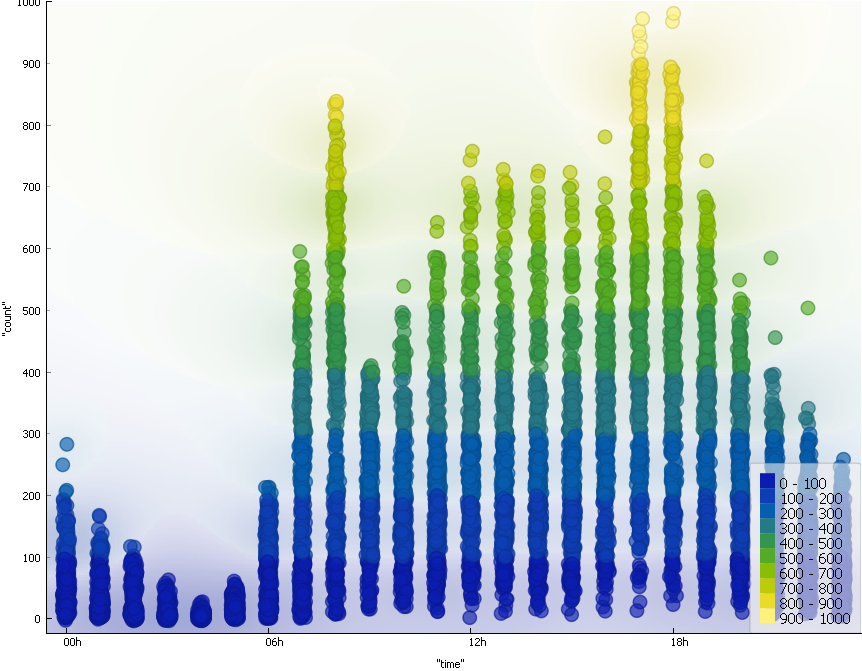
\includegraphics[scale=0.4] {graf}
		\caption{\label{fig:1} A visualization of the bikes in use in its relation to time of day. The plot clearly indicates hourly trends, showing that bike demand goes up around 8:00 and 16:00.}
	\end{figure}
	
	In my future work I will categorize the \textit{time} variable and see if forecasting of the bike sharing will be better ot worse based on whether the variable time is numeric or categorical.
	
	
	
	\section{Future work}
	I will use five different machine learning methods (linear regression, random forest, kNN, gradient boosting, neural network) on the data set described above to try to forecast hourly use of a Washington's bikeshare system. I will also program one of them from the stratch. I will try to optimize every mentioned method by determining  appropriate parameter values using cross-validation and using different columns of data. I will compare methods by calculating different errors (MSE, RMSE, MAE, R2).
	

	

	
	
	% --------------------------------------------------------------
	%     You don't have to mess with anything below this line.
	% --------------------------------------------------------------
	
	
\end{document}